%% Exemplo de utilizacao do estilo de formatacao normas-utf-tex (http://normas-utf-tex.sourceforge.net)
%% Autores: (200?-2011) Hugo Vieira Neto (hvieir@utfpr.edu.br)
%%          (200?-2011) Diogo Rosa Kuiaski (diogo.kuiaski@gmail.com)
%%          (2011-2012) Marcos Talau <talau@users.sourceforge.net>
%% Colaborador:
%%          (2011) César M. Vargas Benitez <cesarvargasb@gmail.com>
%%          (2015) Glauber Gomes de Oliveira Brante <gbrante@utfpr.edu.br>

\documentclass[openright]{normas-utf-tex} %openright = o capitulo comeca sempre em paginas impares
%\documentclass[oneside]{normas-utf-tex} %oneside = para documentos com numero de paginas menor que 100 (apenas frente da folha)

% force A4 paper format
\special{papersize=210mm,297mm}
\usepackage[plainpages=true, bookmarks=true, breaklinks, pdfstartview=FitH,pdftitle={Nome da Teste},pdfauthor={Nome do autor},pdfsubject={Assunto do documento},pdfkeywords={Palavras-chave}]{hyperref}
\usepackage[hyphenbreaks]{breakurl}
\urlstyle{same}
%configuracao correta das referencias bibliograficas.
\usepackage[alf,abnt-emphasize=bf,bibjustif,recuo=0cm,abnt-etal-cite=2,abnt-etal-list=0,abnt-thesis-year=both]{abntcite}
\usepackage[brazil]{babel} % pacote portugues brasileiro
\usepackage[utf8]{inputenc} % pacote para acentuacao direta

\usepackage{amsmath,amsfonts,amssymb} % pacote matematico
\usepackage{graphicx} % pacote grafico
%\usepackage{times} % fonte times (substituida pelos dois comandos abaixo - padrao LATEX)
\usepackage[T1]{fontenc}
\usepackage{lmodern}
\usepackage[final]{pdfpages} % adicao da ata
\usepackage{float}

% ---------- Preambulo ----------
\instituicao{Universidade Tecnológica Federal do Paraná} % nome da instituicao
\programa{Programa de Pós-graduação em Sistemas de Energia} % nome do programa
\area{Automação e Sistemas de Energia} % area de concentracao

\documento{Dissertação} % [Dissertacao] ou [Tese]
\documentoingles{Thesis}
\nivel{Mestrado} % [Mestrado] ou [Doutorado]
\titulacao{Mestre} % [Mestre] ou [Doutor]

\titulo{Título em Português} % titulo do trabalho em portugues
\title{Title in English} % titulo do trabalho em ingles

\autor{Nome Completo} % autor do trabalho
\cita{SOBRENOME, Nome} % sobrenome (maiusculas), nome do autor do trabalho

\palavraschave{Palavra-chave 1. Palavra-chave 2. ...} % palavras-chave do trabalho
\keywords{Keyword 1. Keyword 2. ...} % palavras-chave do trabalho em ingles

\comentario{\UTFPRdocumentodata\ apresentada ao \UTFPRprogramadata\ da \ABNTinstituicaodata\ como requisito parcial para obtenção do título de ``\UTFPRtitulacaodata\ em Engenharia Elétrica'' -- Área de Concentração: \UTFPRareadata.}

\orientador{Nome do Orientador} % nome do orientador do trabalho
%\orientador[Orientadora:]{Nome da Orientadora} % <- no caso de orientadora, usar esta sintaxe
\coorientador{Nome do Coorientador} % nome do coorientador do trabalho, caso exista
%\coorientador[Coorientadora:]{Nome da Coorientadora} % <- no caso de co-orientadora, usar esta sintaxe

\local{Curitiba} % cidade
\data{2020} % ano


% desativa hifenizacao mantendo o texto justificado.
\tolerance=1
\emergencystretch=\maxdimen
\hyphenpenalty=10000
\hbadness=10000
\sloppy


%---------- Inicio do Documento ----------
\begin{document}
\pdfstringdefDisableCommands{%
	\let\MakeUppercase\relax
}
\capa % geracao automatica da capa
\folhaderosto % geracao automatica da folha de rosto


% insercao da ATA
%\includepdf{ata.pdf}


% dedicatoria
\begin{dedicatoria}
Texto da dedicat\'oria.
\end{dedicatoria}

% agradecimentos (opcional)
\begin{agradecimentos}
Texto dos agradecimentos.
\end{agradecimentos}

% epigrafe (opcional)
\begin{epigrafe}
Texto da ep\'igrafe.
\end{epigrafe}

%resumo
\begin{resumo}
Texto do resumo (m\'aximo de 500 palavras).
\end{resumo}

%abstract
\begin{abstract}
Abstract text (maximum of 500 words).
\end{abstract}

% listas (opcionais, mas recomenda-se a partir de 5 elementos)
\listadefiguras % geracao automatica da lista de figuras
\listadetabelas % geracao automatica da lista de tabelas
%\listadequadros % adivinhe :)
\listadesiglas % geracao automatica da lista de siglas
\listadesimbolos % geracao automatica da lista de simbolos

% sumario
\sumario % geracao automatica do sumario

% Pacotes necessários quando não se usa sumário
%\renewcommand{\chaptertitlepagestyle}{plainheader}
%\pagenumbering{arabic}



%---------- Inicio do Texto ----------
% recomenda-se a escrita de cada capitulo em um arquivo texto separado (exemplo: intro.tex, fund.tex, exper.tex, concl.tex, etc.) e a posterior inclusao dos mesmos no mestre do documento utilizando o comando \input{}, da seguinte forma:
%\input{intro.tex}
%\input{fund.tex}
%\input{exper.tex}
%\input{concl.tex}


%\setcounter{page}{12}

%---------- Primeiro Capitulo ----------
\chapter{Introdução}
\label{chap:introducao}

O presente documento é um exemplo de uso do estilo de formatação \LaTeX\ elaborado para atender às Normas para Elaboração de Trabalhos Acadêmicos da UTFPR. O estilo de formatação {\ttfamily normas-utf-tex.cls} tem por base o pacote \textsc{abn}\TeX~-- cuja leitura da documentação \cite{abnTeX2009} é fortemente sugerida~-- e o estilo de formatação \LaTeX\ da UFPR.

Para melhor entendimento do uso do estilo de formatação {\ttfamily normas-utf-tex.cls}, aconselha-se que o potencial usuário analise os comandos existentes no arquivo \TeX\ ({\ttfamily modelo\_*.tex}) e os resultados obtidos no arquivo PDF ({\ttfamily modelo\_*.pdf}) depois do processamento pelo software \LaTeX\ + \textsc{Bib}\TeX~\cite{LaTeX2009,BibTeX2009}. Recomenda-se a consulta ao material de referência do software para a sua correta utilização~\cite{Lamport1986,Buerger1989,Kopka2003,Mittelbach2004}.

\section{Motivação}
\label{sec:motivacao}

Uma das principais vantagens do uso do estilo de formatação {\ttfamily normas-utf-tex.cls} para \LaTeX\ é a formatação \textit{automática} dos elementos que compõem um documento acadêmico, tais como capa, folha de rosto, dedicatória, agradecimentos, epígrafe, resumo, abstract, listas de figuras, tabelas, siglas e símbolos, sumário, capítulos, referências, etc. Outras grandes vantagens do uso do \LaTeX\ para formatação de documentos acadêmicos dizem respeito à facilidade de gerenciamento de referências cruzadas e bibliográficas, além da formatação~-- inclusive de equações  matemáticas~-- correta e esteticamente perfeita.

\section{Objetivos}
\label{sec:objetivos}

\subsection{Objetivo Geral}
\label{subsec:objetivoGeral}

Prover um modelo de formatação \LaTeX\ que atenda às Normas para Elaboração de Trabalhos Acadêmicos da UTFPR~\cite{UTFPR2008}.

\subsection{Objetivos Específicos}
\label{subsec:objetivosEspecificos}

\begin{itemize}
	\item Obter documentos acadêmicos automaticamente formatados com correção e perfeição estética.
	\item Desonerar autores da tediosa tarefa de formatar documentos acadêmicos, permitindo sua concentração no conteúdo do mesmo.
	\item Desonerar orientadores e examinadores da tediosa tarefa de conferir a formatação de documentos acadêmicos, permitindo sua concentração no conteúdo do mesmo.
\end{itemize}



%---------- Segundo Capitulo ----------
\chapter{Desenvolvimento}
\label{chap:desenv}

A seguir ilustra-se a forma de incluir figuras, tabelas, equações, siglas e símbolos no documento, obtendo indexação automática em suas respectivas listas. A numeração sequencial de figuras, tabelas e equações ocorre de modo automático. Referências cruzadas são obtidas através dos comandos {\ttfamily \textbackslash label\{\}} e {\ttfamily \textbackslash ref\{\}}. Por exemplo, não é necessário saber que o número deste capítulo é~\ref{chap:desenv} para colocar o seu número no texto. Isto facilita muito a inserção, remoção ou relocação de elementos numerados no texto (fato corriqueiro na escrita e correção de um documento acadêmico) sem a necessidade de renumerá-los todos.

\section{Figuras}
\label{sec:figuras}

Na figura~\ref{fig:dummy} é apresentado um exemplo de gráfico flutuante. Esta figura aparece automaticamente na lista de figuras. Para uso avançado de gráficos no \LaTeX, recomenda-se a consulta de literatura especializada~\cite{Goossens2007}.

\begin{figure}[!htb]
	\centering
	\caption[Exemplo de uma figura]{Exemplo de uma figura onde aparece uma imagem sem nenhum significado especial.}
	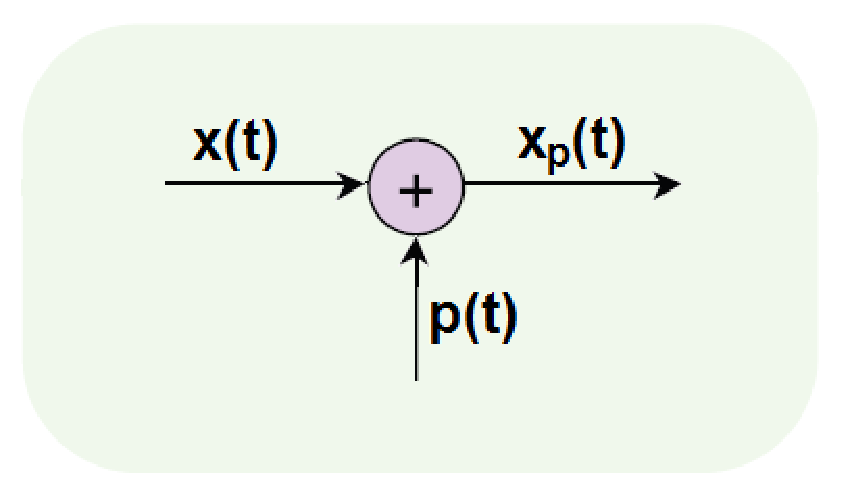
\includegraphics[width=5cm]{./dummy.eps} % <- formatos PNG, EPS e PDF	
	\fonte{Adaptado de \cite{abnTeX2009}}
	\label{fig:dummy}
\end{figure}


\section{Tabelas}
\label{sec:tabelas}

Também é apresentado o exemplo da tabela~\ref{tab:correlacao}, que aparece automaticamente na lista de tabelas. Informações sobre a construção de tabelas no \LaTeX\ podem ser encontradas na literatura especializada~\cite{Lamport1986,Buerger1989,Kopka2003,Mittelbach2004}.

\begin{table}[!htb]
	\centering
	\caption[Exemplo de uma tabela]{Exemplo de uma tabela mostrando a correlação entre x e y.}
	\label{tab:correlacao}
	\begin{tabular}{cc}
		\hline
		x & y \\
		\hline
		1 & 2 \\
		3 & 4 \\
		5 & 6 \\
		7 & 8 \\
		\hline
	\end{tabular}
	\fonte{Autoria própria.}
\end{table}



\section{Equações}
\label{sec:equacoes}

A transformada de Laplace é dada na equação~\eqref{eq:laplace}, enquanto a equação~\eqref{eq:dft} apresenta a formulação da transformada discreta de Fourier bidimensional\footnote{Deve-se reparar na formatação esteticamente perfeita destas equações!}.

\begin{equation}
X(s) = \int\limits_{t = -\infty}^{\infty} x(t) \, \text{e}^{-st} \, dt
\label{eq:laplace}
\end{equation}

\begin{equation}
F(u, v) = \sum_{m = 0}^{M - 1} \sum_{n = 0}^{N - 1} f(m, n) \exp \left[ -j 2 \pi \left( \frac{u m}{M} + \frac{v n}{N} \right) \right]
\label{eq:dft}
\end{equation}

\section{Siglas e símbolos}
\label{sec:siglasSimbolos}

O pacote \textsc{abn}\TeX\ permite ainda a definição de siglas e símbolos com indexação automática através dos comandos {\ttfamily \textbackslash sigla\{\}\{\}} e {\ttfamily \textbackslash simbolo\{\}\{\}}. Por exemplo, o significado das siglas \sigla{PPGSE}{Programa de Pós-graduação em Sistemas de Energia}, \sigla{DAELT}{Departamento Acadêmico de Eletrotécnica} e \sigla{UTFPR}{Universidade Tecnológica Federal do Paraná} aparecem automaticamente na lista de siglas, bem como o significado dos símbolos \simbolo{$\lambda$}{comprimento de onda}, \simbolo{$v$}{velocidade} e \simbolo{$f$}{frequência} aparecem automaticamente na lista de símbolos. Mais detalhes sobre o uso destes e outros comandos do \textsc{abn}\TeX\ são encontrados na sua documentação específica~\cite{abnTeX2009}.


%---------- Terceiro Capitulo ----------
\chapter{Conclusão}
\label{chap:conclusao}

Espera-se que o uso do estilo de formatação \LaTeX\ adequado às Normas para Elaboração de Trabalhos Acadêmicos da UTFPR ({\ttfamily normas-utf-tex.cls}) facilite a escrita de documentos no âmbito desta instituição e aumente a produtividade de seus autores. Para usuários iniciantes em \LaTeX, além da bibliografia especializada já citada, existe ainda uma série de recursos~\cite{CTAN2009} e fontes de informação~\cite{TeX-Br2009,Wikibooks2009} disponíveis na Internet.

Recomenda-se o editor de textos Kile como ferramenta de composição de documentos em \LaTeX\ para usuários Linux. Para usuários Windows recomenda-se o editor \TeX nicCenter~\cite{TeXnicCenter2009} ou TexMaker. O \LaTeX\ normalmente já faz parte da maioria das distribuições Linux, mas no sistema operacional Windows é necessário instalar o software \textsc{MiK}\TeX~\cite{MiKTeX2009}.

Além disso, recomenda-se o uso de um gerenciador de referências como o JabRef~\cite{JabRef2009} ou Mendeley~\cite{Mendeley2009} para a catalogação bibliográfica em um arquivo \textsc{Bib}\TeX, de forma a facilitar citações através do comando {\ttfamily \textbackslash cite\{\}} e outros comandos correlatos do pacote \textsc{abn}\TeX. A lista de referências deste documento foi gerada automaticamente pelo software \LaTeX\ + \textsc{Bib}\TeX\ a partir do arquivo {\ttfamily reflatex.bib}, que por sua vez foi composto com o gerenciador de referências JabRef.

O estilo de formatação \LaTeX\ da UTFPR e este exemplo de utilização foram elaborados por Diogo Rosa Kuiaski (diogo.kuiaski@gmail.com) e Hugo Vieira Neto (hvieir@utfpr.edu.br), com contribuições de César Vargas Benitez. A adaptação para o PPGSE foi feita por Glauber Brante (gbrante@utfpr.edu.br). Sugestões de melhorias são bem-vindas.



%---------- Referencias ----------
\clearpage % this is need for add +1 to pageref of bibstart used in 'ficha catalografica'.
\label{bibstart}
\bibliography{reflatex} % geracao automatica das referencias a partir do arquivo reflatex.bib
\label{bibend}


%---------- Apendices (opcionais) ----------
\apendice
\chapter{Nome do Apêndice}
\label{chap:apendice}

Use o comando {\ttfamily \textbackslash apendice} e depois comandos {\ttfamily \textbackslash chapter\{\}}
para gerar títulos de apêndices.


% ---------- Anexos (opcionais) ----------
\anexo
\chapter{Nome do Anexo}
\label{chap:anexo}

Use o comando {\ttfamily \textbackslash anexo} e depois comandos {\ttfamily \textbackslash chapter\{\}}
para gerar títulos de anexos.


% --------- Ordenacao Afabetica da Lista de siglas --------
%\textbf{* Observa\c{c}\~oes:} a ordenacao alfabetica da lista de siglas ainda nao eh realizada de forma automatica, porem
% eh possivel se de realizar isto manualmente. Duas formas:
%
% ** Primeira forma)
%    A ordenacao eh feita com o auxilio do comando 'sort', disponivel em qualquer
% sistema Linux e UNIX, e tambem em sistemas Windows se instalado o coreutils (http://gnuwin32.sourceforge.net/packages/coreutils.htm)
% comandos para compilar e ordenar, supondo que seu arquivo se chame 'dissertacao.tex':
%
%      $ latex dissertacao
%      $ bibtex dissertacao && latex dissertacao
%      $ latex dissertacao
%      $ sort dissertacao.lsg > dissertacao.lsg.tmp
%      $ mv dissertacao.lsg.tmp dissertacao.lsg
%      $ latex dissertacao
%      $ dvipdf dissertacao.dvi
%
%
% ** Segunda forma)
%\textbf{Sugest\~ao:} crie outro arquivo .tex para siglas e utilize o comando \sigla{sigla}{descri\c{c}\~ao}.
%Para incluir este arquivo no final do arquivo, utilize o comando \input{arquivo.tex}.
%Assim, Todas as siglas serao geradas na ultima pagina. Entao, devera excluir a ultima pagina da versao final do arquivo
% PDF do seu documento.


%-------- Citacoes ---------
% - Utilize o comando \citeonline{...} para citacoes com o seguinte formato: Autor et al. (2011).
% Este tipo de formato eh utilizado no comeco do paragrafo. P.ex.: \citeonline{autor2011}

% - Utilize o comando \cite{...} para citacoeses no meio ou final do paragrafo. P.ex.: \cite{autor2011}



%-------- Titulos com nomes cientificos (titulo, capitulos e secoes) ----------
% Regra para escrita de nomes cientificos:
% Os nomes devem ser escritos em italico,
%a primeira letra do primeiro nome deve ser em maiusculo e o restante em minusculo (inclusive a primeira letra do segundo nome).
% VEJA os exemplos abaixo.
%
% 1) voce nao quer que a secao fique com uppercase (caixa alta) automaticamente:
%\section[nouppercase]{\MakeUppercase{Estudo dos efeitos da radiacao ultravioleta C e TFD em celulas de} {\textit{Saccharomyces boulardii}}
%
% 2) por padrao os cases (maiusculas/minuscula) sao ajustados automaticamente, voce nao precisa usar makeuppercase e afins.
% \section{Introducao} % a introducao sera posta no texto como INTRODUCAO, automaticamente, como a norma indica.


\end{document}
